\chapter{Aplikacja}
\section{Opis działania aplikacji}
Głównym założeniem aplikacji wizualizującej pracę systemu było zaprezentowanie pracy sytemu w sposób przejrzysty i uporządkowany. Dodatkowo aplikacja powinna umożliwiać zmianę wybranych parametrów systemy oraz zapewniać jednoczesny dostęp dla wielu użytkowników. Biorąc pod uwagę wymienione wymagania zdecydowano się na napisanie aplikacji webowej wykorzystując do tego celu framework \textit{Angular 4 - https://angular.io/}.
\section{Opis okien}
Aplikacja do wizualizacji pracy systemu podzielona jest na 5 ekranów. 
\begin{enumerate}
	\item \textbf{Schemat} - przedstawia schemat rozpatrywanej instalacji,
	\item \textbf{Statystyki} - przedstawia najważniejsze dane opisujące aktualny stan instalacji takie jak: poziomu cieczy w każdym ze zbiorników, aktualne stężenie, a także przebiegi czasowe tych sygnałów zaprezentowane za pomocą wykresów,
	\item \textbf{Obiekt} - prezentuje szczegółowe dane dotyczące obiektu regulacji oraz daje możliwość zmieniania limitów w każdym ze zbiorników.
	\item \textbf{Regulator} - przedstawia przebiegi czasowe sygnałów sterowania, a także daje możliwość zmieniania nastaw regulatorów,
	\item \textbf{Logi} - daje możliwość generowania raportów z wybranych stanów pracy systemu tzn: zwykła praca, stany alarmowe, zmiany wartości parametrów systemu.
\end{enumerate}
Każdy z ekranów na składa się z trzech głównych części \ref{fig:sc0}:
\begin{enumerate}
	\item Pasek menu - umożliwia przechodzenie pomiędzy wszystkimi oknami aplikacji,
	\item \textbf{Panel danych} - w jego obszarze wyświetlane są dane dotyczące poszczególnych funkcjonalności systemu,
	\item \textbf{Pasek wiadomości} - Wyświetlane są na nim najważniejsze wiadomości dotyczące pracy systemu takie jak np. przekroczenie limitów.
\end{enumerate}

\section{Alarmy}
Każdy zbiornik ma zdefiniowany zestaw czterech limitów poziomu cieczy tzn. 
\begin{enumerate}
	\item Limit minimalny krytyczny,
	\item Limit minimalny,
	\item Limit maksymalny,
	\item Limit maksymalny krytyczny
\end{enumerate}
Wartości wyżej wymienionych limitów mogą być monitorowane oraz zmieniane przy wykorzystaniu ekranu \textit{Obiekty}. Każda zmiana wartości jest automatycznie zapisywana w bazie danych i propagowana do regulatora.

W aplikacji zaimplementowano również propagację alarmów. W momencie przekroczenia dowolnego ze zdefiniowanych limitów pod wskazany adres wysyłany jest email informujący o tym zdarzeniu. 

\section{Regulatory}
Aplikacja daje możliwość operatorowi na zdalną zmianę parametrów regulatorów za pomocą ekranu \textit{Regulator}. Podobnie jak w przypadku alarmów każdorazowa zmiana dowolnego parametru jest propagowana do regulatora i zapisywana w bazie danych.
\section{Wygląd aplikacji}
Na poniższych rysunkach przedstawiono screen-y z działania opisywanej aplikacji dla każdego z dostępnych ekranów.
\begin{figure}[H]
	\centering
	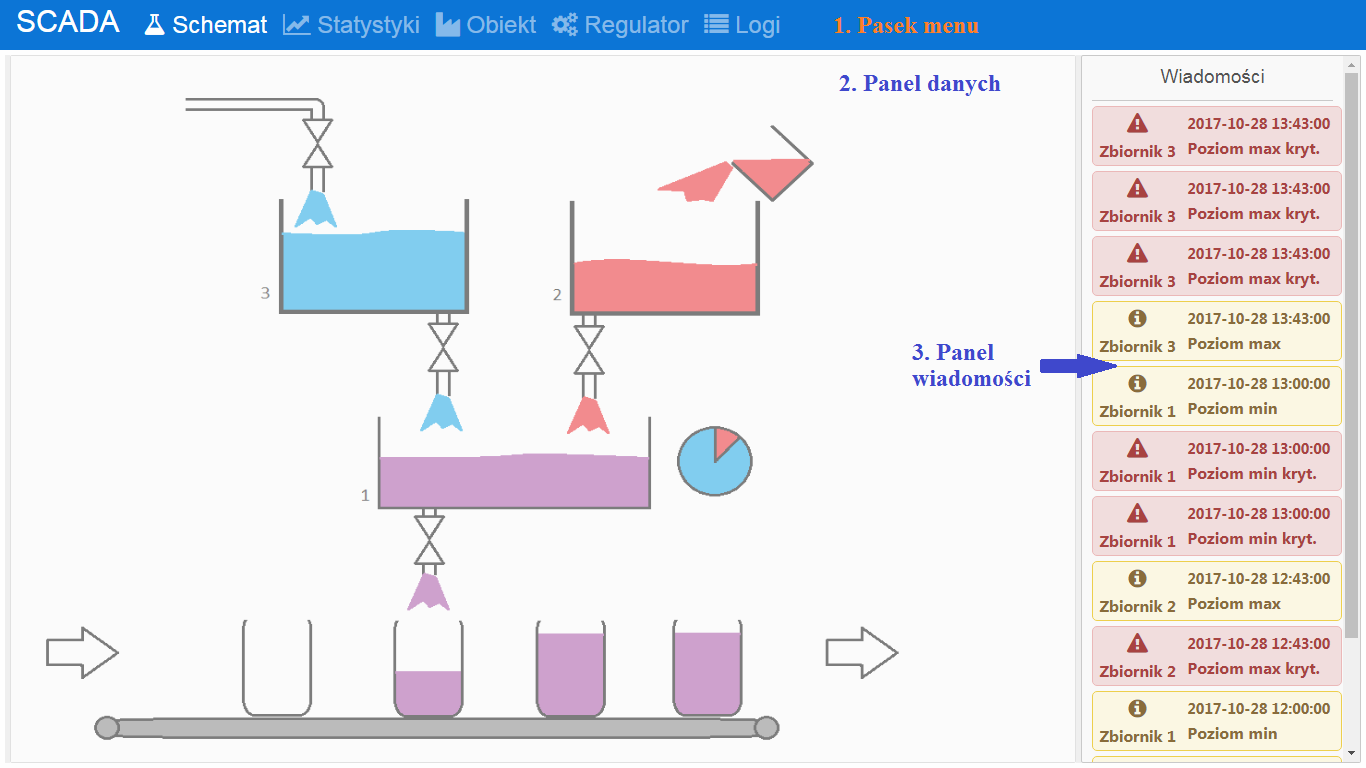
\includegraphics[scale = 0.45]{fig/sc0.png}
	\caption{Budowa ekranu.}
	\label{fig:sc0}
\end{figure}


\begin{figure}[H]
	\centering
	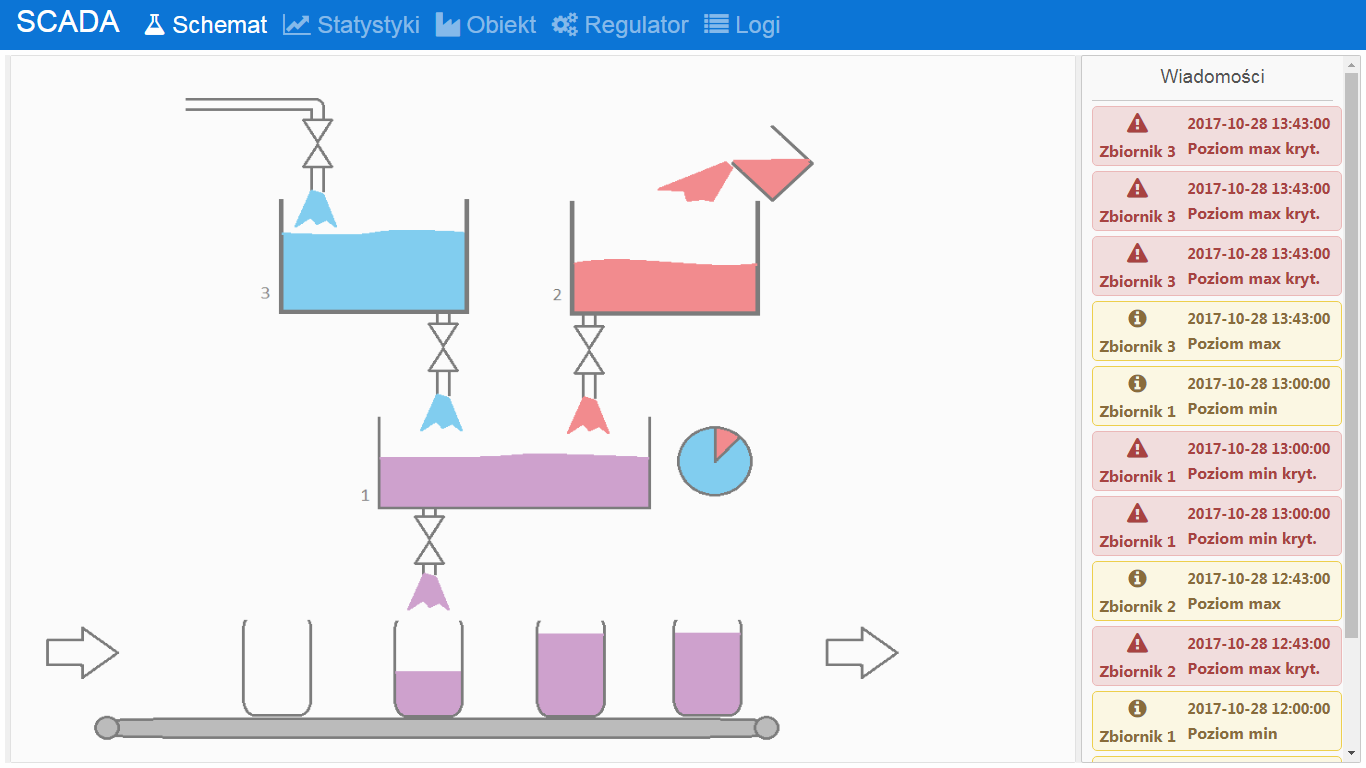
\includegraphics[scale = 0.45]{fig/sc1.png}
	\caption{Schemat systemu.}
	\label{fig:sc1}
\end{figure}

\begin{figure}[H]
	\centering
	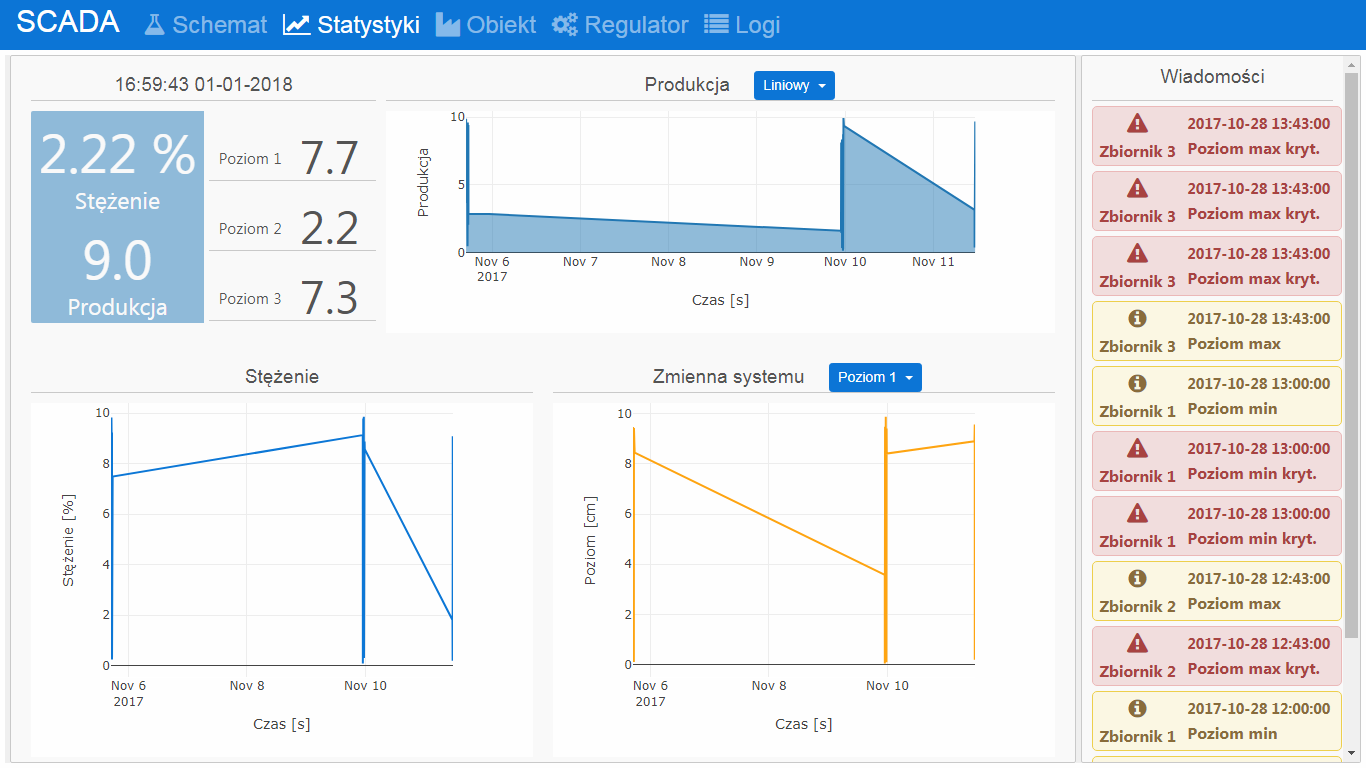
\includegraphics[scale = 0.45]{fig/sc2.png}
	\caption{Statystyki systemu.}
	\label{fig:sc2}
\end{figure}

\begin{figure}[H]
	\centering
	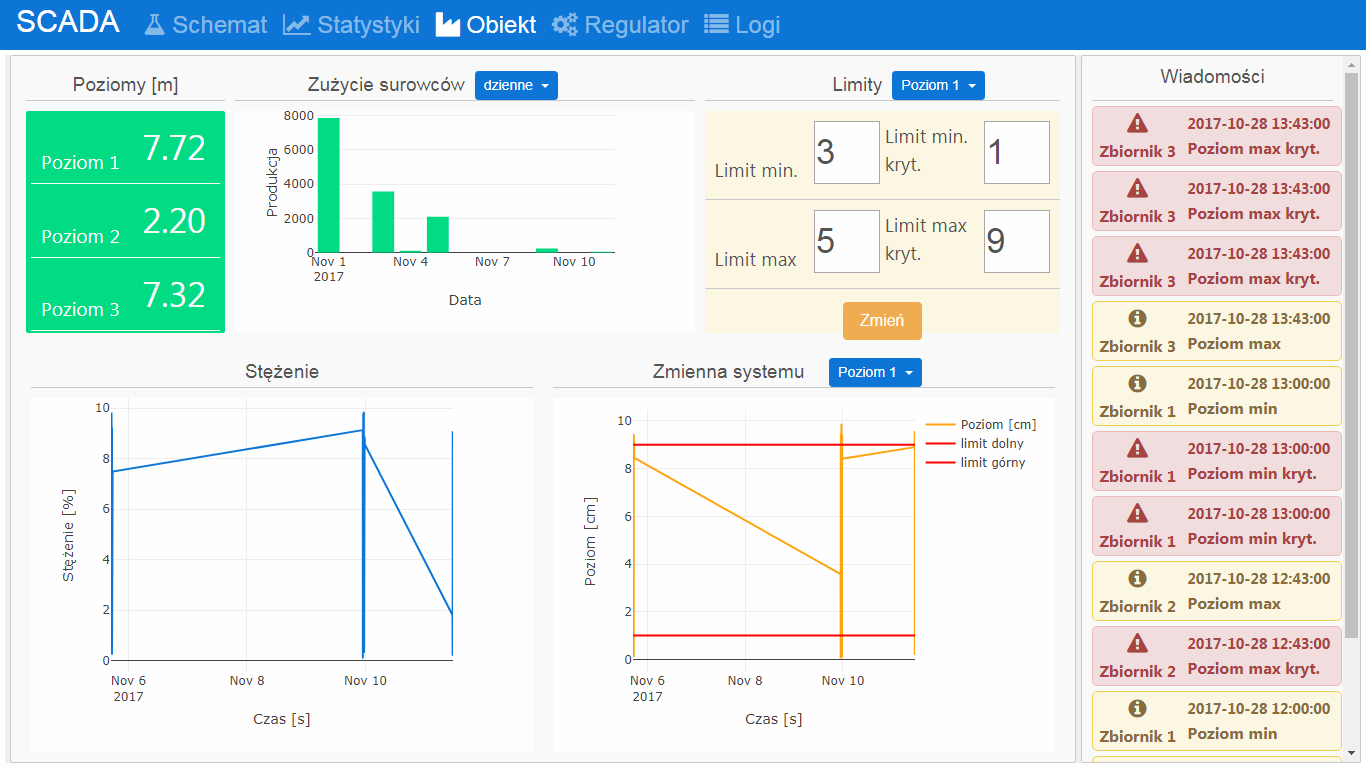
\includegraphics[scale = 0.5]{fig/sc3.png}
	\caption{Ekran przedstawiający stan instalacji.}
	\label{fig:sc3}
\end{figure}

\begin{figure}[H]
	\centering
	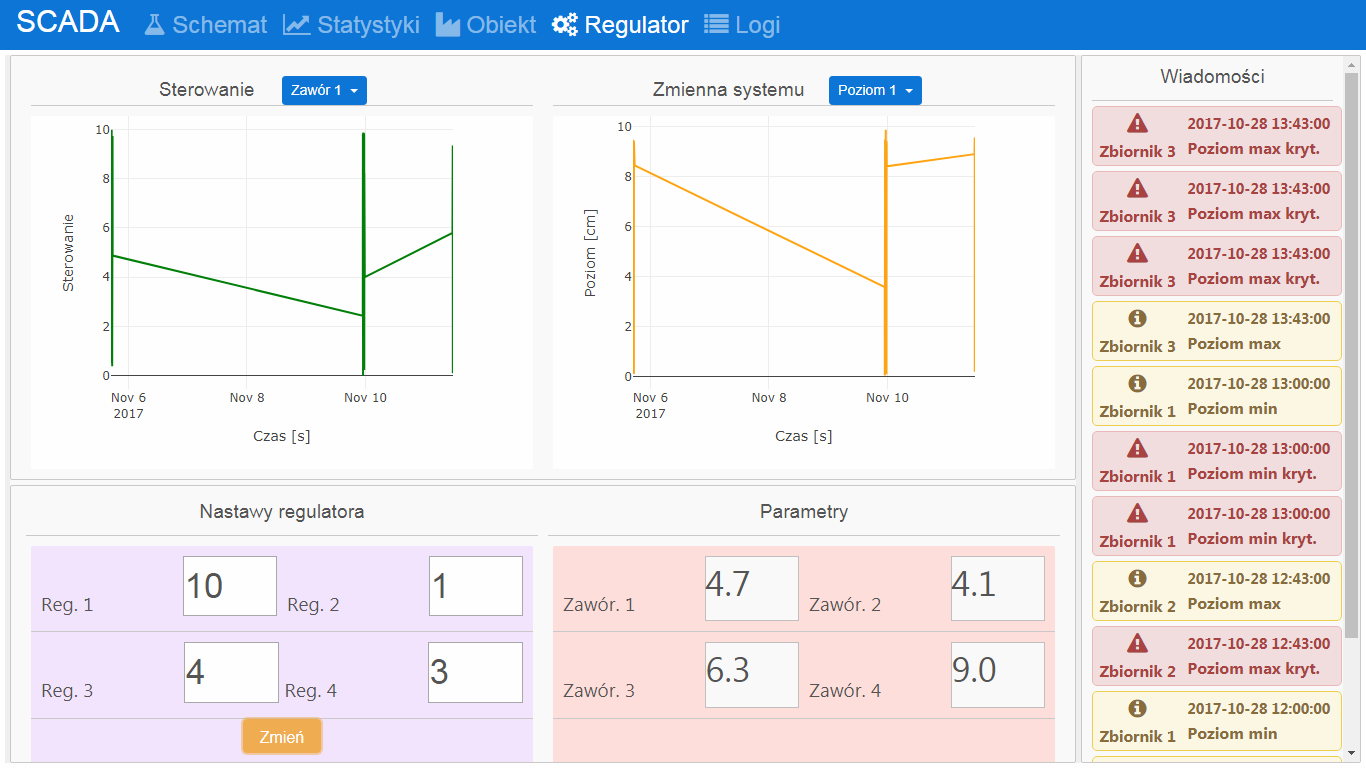
\includegraphics[scale = 0.5]{fig/sc4.png}
	\caption{Ekran przestawiający pracę regulatorów.}
	\label{fig:sc4}
\end{figure}

\begin{figure}[H]
	\centering
	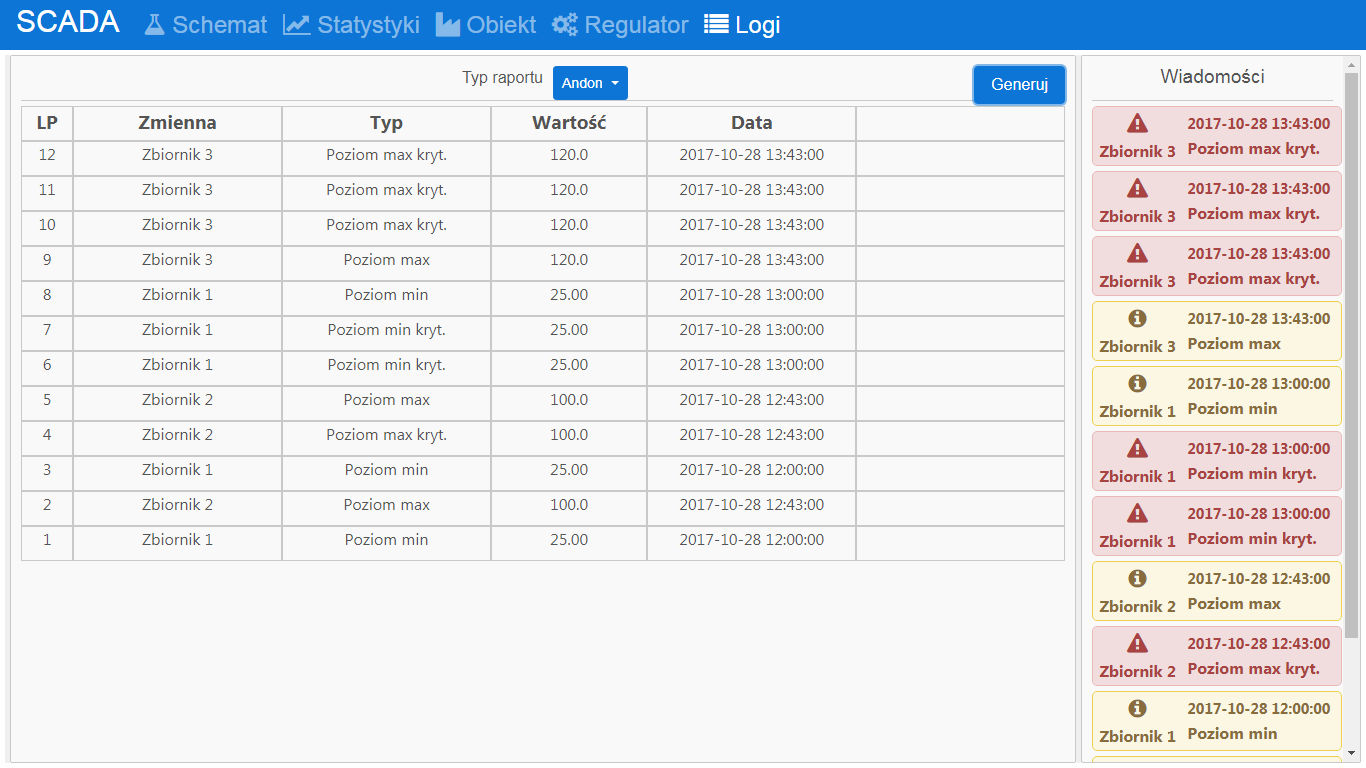
\includegraphics[scale = 0.5]{fig/sc5.png}
	\caption{Ekran do generowania raportów.}
	\label{fig:sc5}
\end{figure}

\section{Uruchomienie aplikacji}
Do uruchomienie aplikacji należy: 
\begin{enumerate}
	\item na wybranym komputerze zainstalować serwer \textit{Node.js - https://nodejs.org/en/}
	\item  pobrać kod \'zródłowy projektu ze strony \textit{https://github.com/maciekc/SCADA2}
	\item w konsoli systemu \textit{Windows} należy przejść do głównego folderu projektu  \textit{SCADA-app} i wywołać procedurę \textbf{npm start}
	\item od tej pory aplikacja będzie dostępna pod adresem \textit{www.localhost:4200}.
	
\end{enumerate}